\chapter{Materiales y Métodos}
\section{Materiales}
\subsection{Datos públicos} 
\label{sec:DatosPublicos}
Para este TFG se han utilizado diversos conjuntos de datos públicos para la 
evaluación y elección de los modelos anteriormente descritos. De entre ellos 
están SJTU\cite{SJTU}, WPC\cite{WPC1,WPC2} y LS-SJTU-PCQA\cite{ResSCNN} que tratan 
de conjuntos de nubes de puntos generalistas, de personas, animales y objetos cotidianos.

El primero de ellos parte de 10 nubes de puntos de referencia, ver Figura \ref{fig:SJTU}, 
a las cuales se aplican 7 tipos de distorsiones. Estas son: compresión, ruido 
al color, ruido geométrico, ruido gaussiano y combinación entre ellas, ver Tabla \ref{tab:SJTU}. Todas se aplican en una escala creciente
de intensidad del 1 al 6. Luego, se obtiene un MOS de 10 individuos para las 420 
nubes de puntos que sirve como medida de calidad de las mismas y para evaluar las predicciones del modelo.

\begin{figure}[htp]
  \centering 
    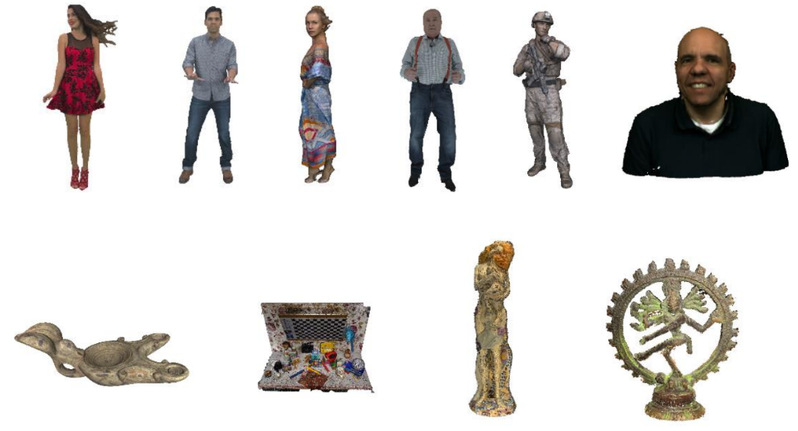
\includegraphics[width=0.95\textwidth]{imagenes/chapter4/SJTU}
    \caption{Ejemplo de conjuntos de datos SJTU\cite{SJTU}.}
    \label{fig:SJTU}
\end{figure}

\begin{table}[htp]
  \centering 
  \scriptsize
  \begin{tabular}{|c|c|}
    \hline
    \rowcolor[HTML]{FFC702}
    \textbf{Número} & \textbf{Tipo de Distorsión} \\ 
    \hline 
    0 & OT: Compresión octree\cite{OctreeCompression} \\ 
    \hline 
    1 & CN: Ruido fotométrico\\ 
    \hline 
    2 & DS: Submuestreo uniforme \\
    \hline 
    3 & DS + CN \\
    \hline 
    4 & DS + GGN \\
    \hline 
    5 & GGN: Ruido geométrico gaussiano \\
    \hline 
    6 & CN + GGN \\ 
    \hline 
  \end{tabular}
  \caption{Ejemplo de distorsiones en SJTU\cite{SJTU}.}
  \label{tab:SJTU}
\end{table}

El segundo dataset, WPC\cite{WPC1, WPC2}, también posee distorsiones como submuestreo uniforme y 
ruido gaussiano (aplicados de manera distinta), pero a su vez posee nuevos tipos 
de distorsiones. Estos son basados en distintos tipos de compresión: V-PCC, G-PCC y \emph{trisoup}.
Además, posee distintos tipos de nubes de puntos, ver Figura \ref{fig:WPC}, que 
pueden influir en el rendimiento del modelo si el conjunto no es
suficientemente amplio y representativo de lo que puede encontrarse una vez entrenado. 

\begin{figure}[htp]
  \begin{center}
    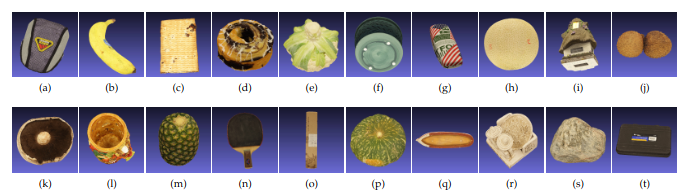
\includegraphics[width=0.95\textwidth]{imagenes/chapter4/WPC}
  \end{center}
  \caption{Ejemplo de conjunto de datos WPC\cite{WPC1, WPC2}.}
  \label{fig:WPC}
\end{figure}

Los dos anteriores han sido utilizados sobre todo para la evaluación y elección 
del modelo de regresión a utilizar. Son los conjuntos de datos más conocidos 
y que habitualmente están presentes en las publicaciones más recientes. Además, se realizaron 
pruebas de ejecuciones de algunos métodos de código abierto para verificar los 
resultados. Sin embargo, es el último es el que finalmente se utiliza para entrenar un modelo para estimar 
la calidad de las imágenes médicas. Esto es porque LS-SJTU-PCQA\cite{ResSCNN} 
es el mayor conjunto de datos 
en el momento de escritura, y posee tipos de distorsiones que pueden simular 
lo que sería ciertos errores y ruidos presentes en imágenes médicas. Por ejemplo, 
el ruido gaussiano (simular errores de transmisión y almacenado de datos), 
rotación y movimiento local (simular el movimiento del paciente) y compresión 
octree y por submuestreo uniforme (algoritmos de compresión comúnmente usados).
Aparte, es el con mayor amplitud de modelos base, con distintos tipos y categorías 
de objetos. Ver Figura \ref{fig:LS-SJTU-PCQA}.

\begin{figure}
  \begin{center}
    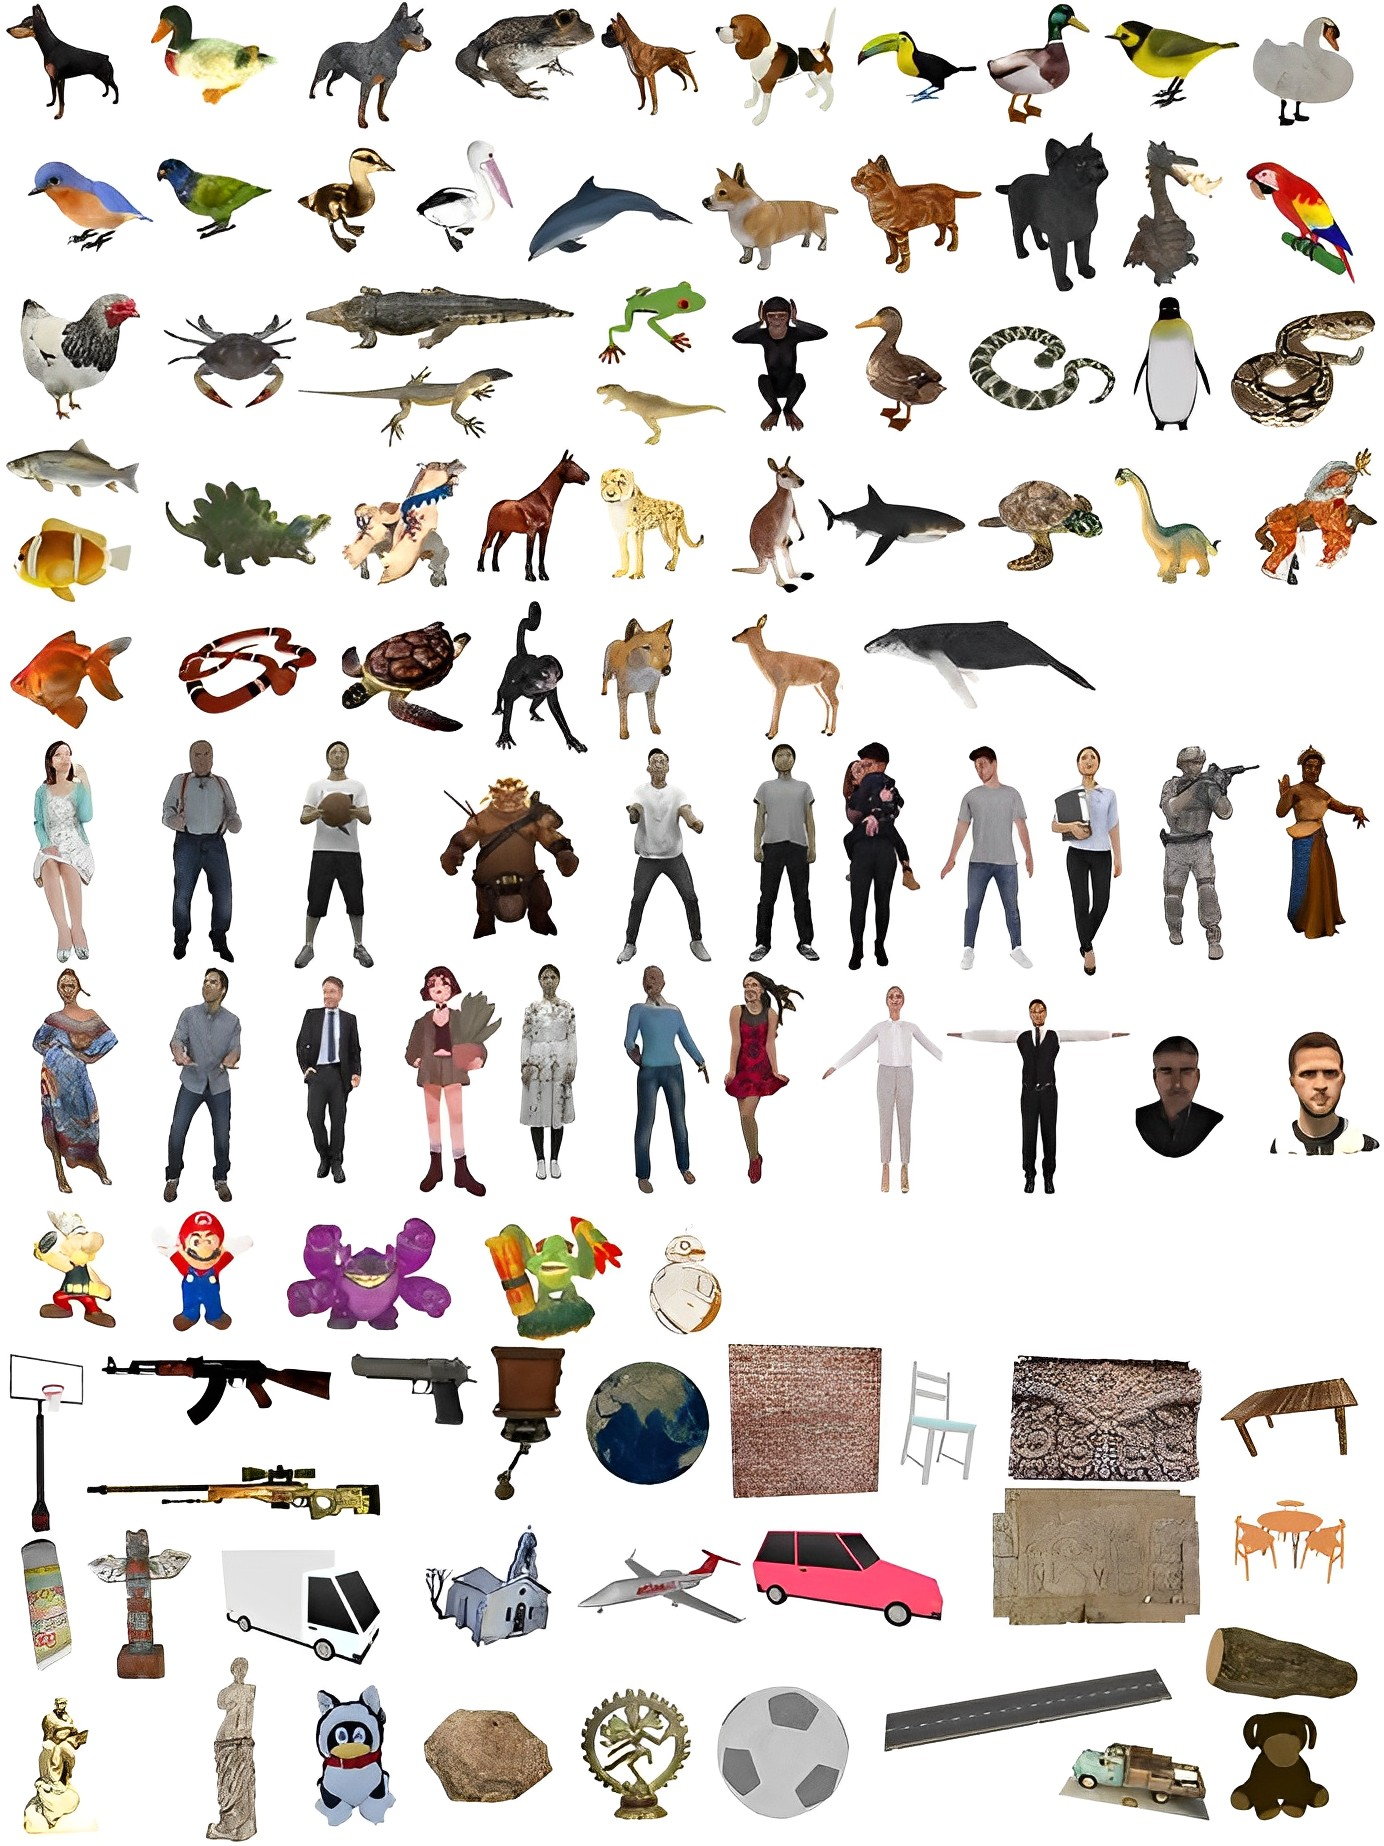
\includegraphics[width=0.95\textwidth]{imagenes/chapter4/LSPCQA}
  \end{center}
  \caption{Ejemplo de conjunto de datos LS-SJTU-PCQA\cite{ResSCNN}.}
  \label{fig:LS-SJTU-PCQA}
\end{figure}

\subsection{Conjunto de datos médicos}
\label{sec:OurData}
Para este TFG se tiene disponible una colección tomografías computerizadas, de distintas
partes del cuerpo, de 2 individuos distintos. 
De los cuales han sido segmentados las clavículas, el seno frontal y los senos maxilares. 
A parte, disponemos de volúmenes del cráneo de otros 3 individuos, una pubis izquierda y
una pubis derecha, ver Figura \ref{fig:OurDataExample}. Es decir, en total disponemos de 11 nubes de puntos de alta 
calidad, que representan distintos volúmenes de exámenes médicos.

\begin{figure}[htp]
  \begin{subfigure}[b]{0.49\textwidth}
  \centering 
  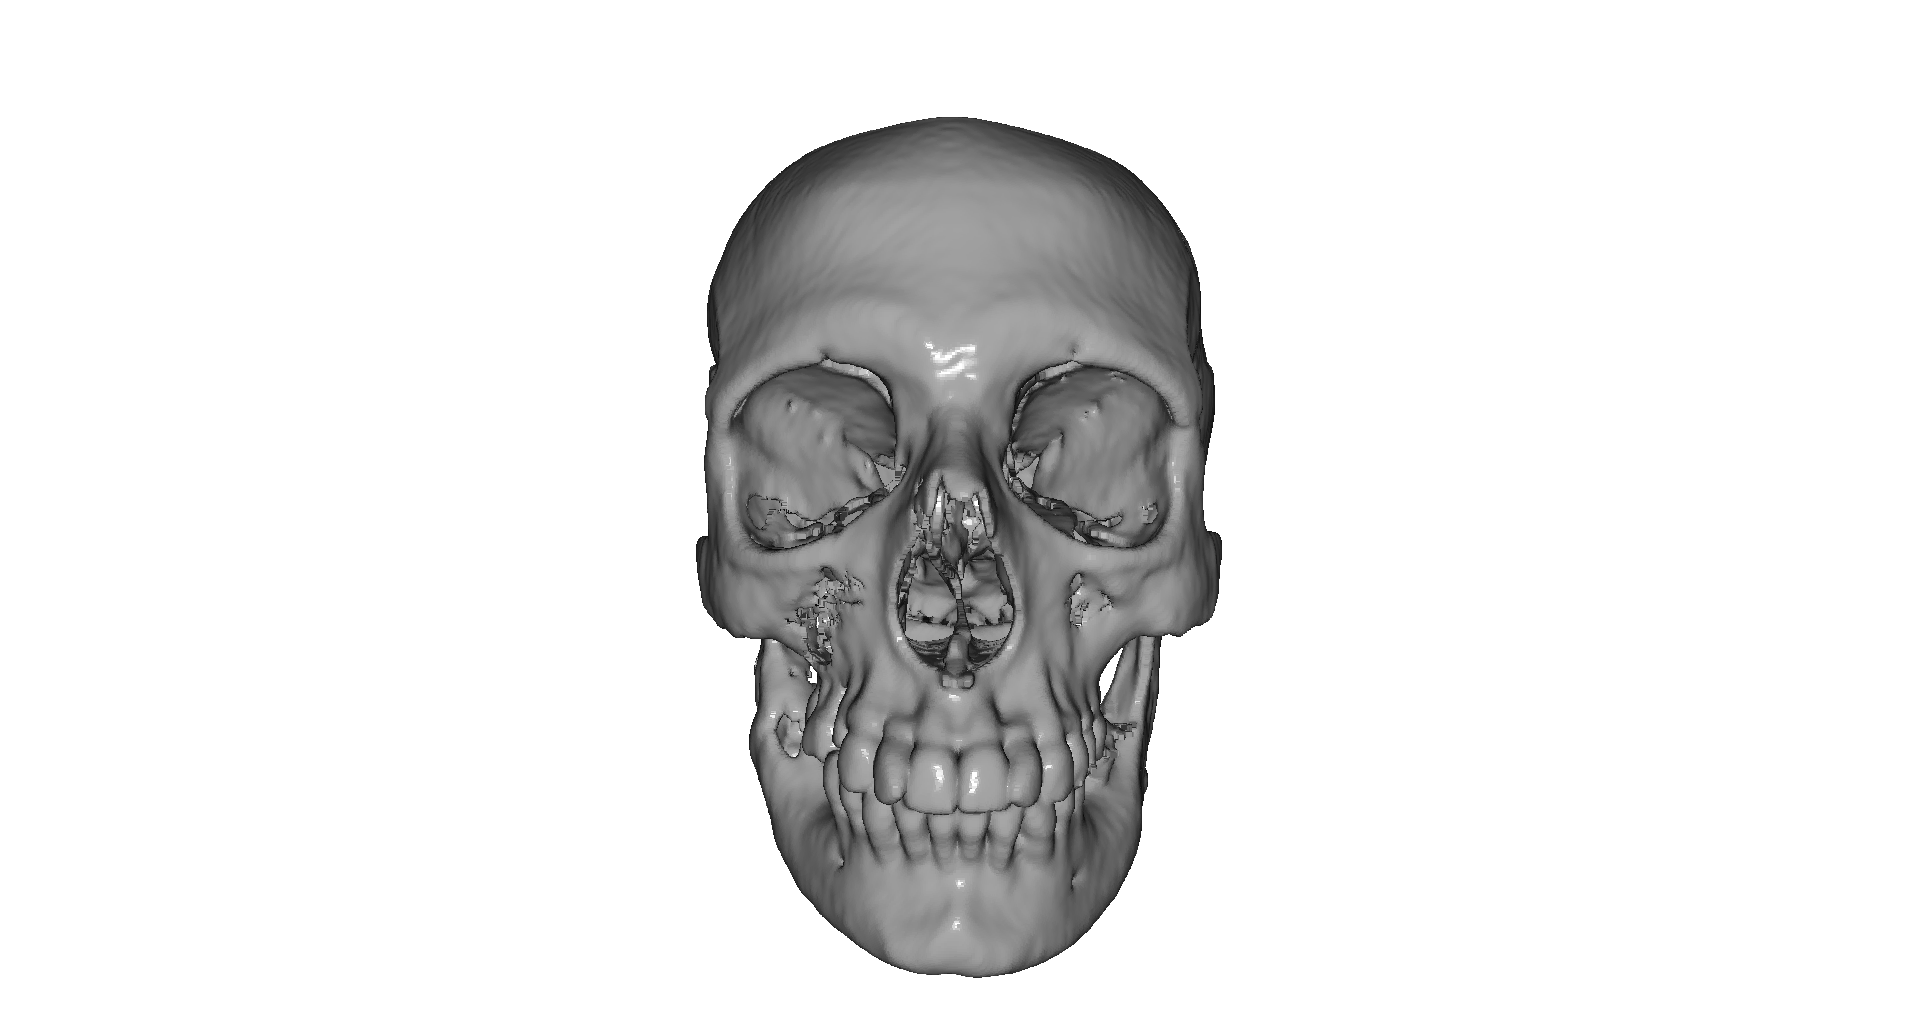
\includegraphics[width=\textwidth]{imagenes/chapter4/Craneo12018377.png}
  \end{subfigure}
  \begin{subfigure}[b]{0.49\textwidth}
  \centering 
  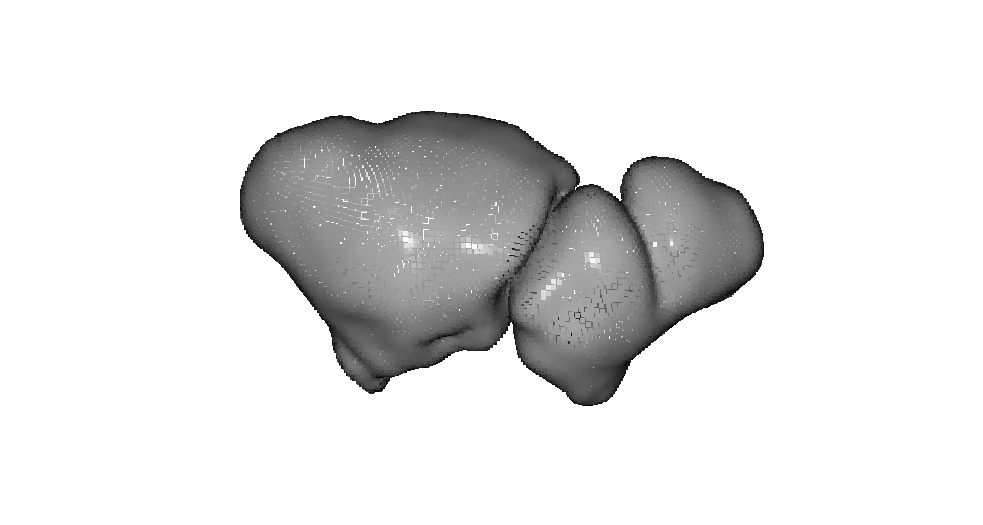
\includegraphics[width=\textwidth]{imagenes/chapter4/SenoFrontal100205.png}
  \end{subfigure}

  \begin{subfigure}[b]{0.49\textwidth}
  \centering 
  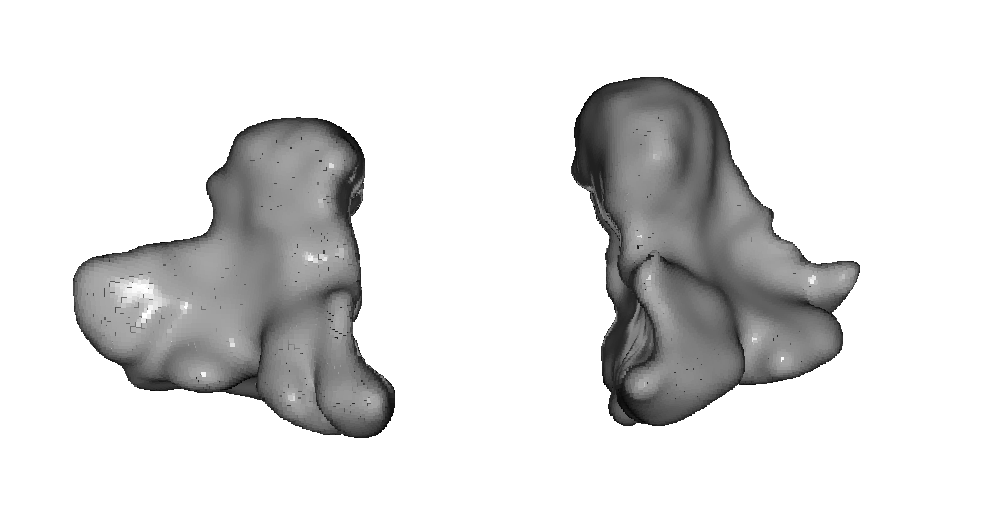
\includegraphics[width=\textwidth]{imagenes/chapter4/Maxilar100205.png}
  \end{subfigure}
  \begin{subfigure}[b]{0.49\textwidth}
  \centering 
  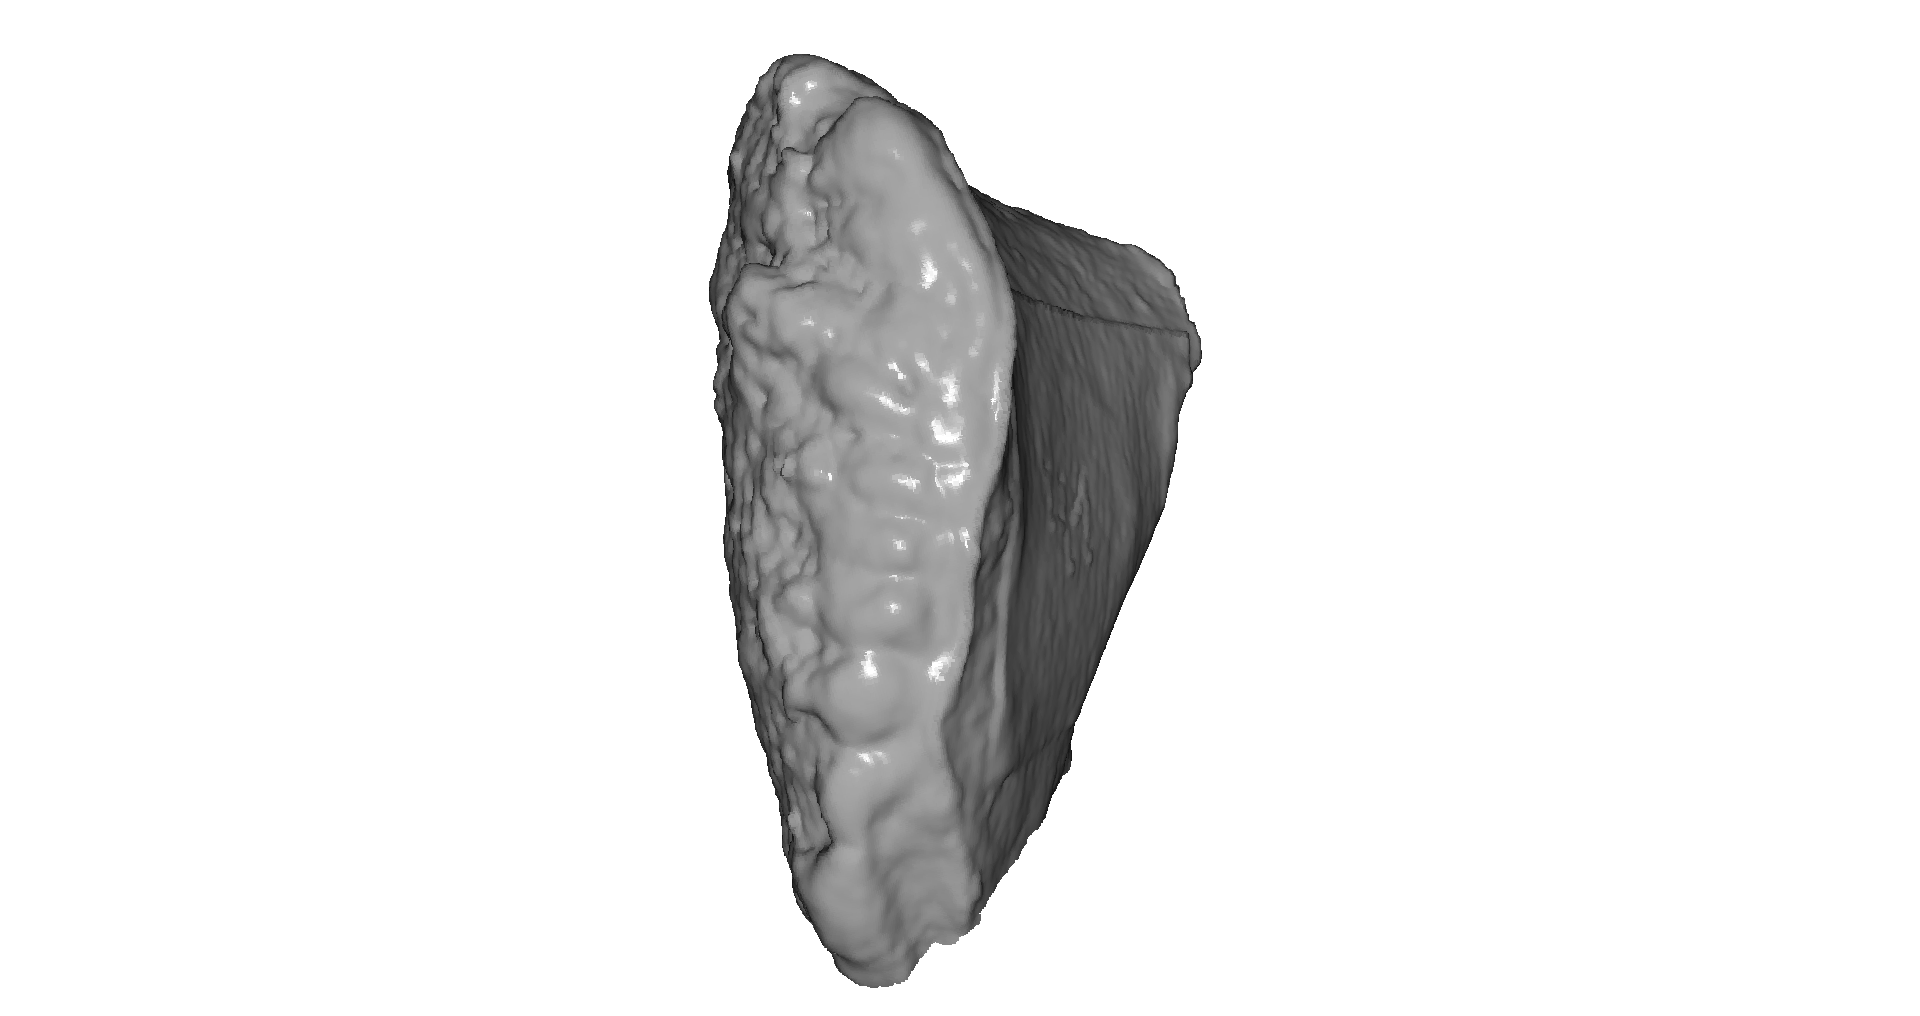
\includegraphics[width=\textwidth]{imagenes/chapter4/PubisDch.png}
  \end{subfigure}
  \caption[Ejemplo de nuestras imágenes médicas]{Ejemplo de nuestras imágenes médicas.
  Arriba a la izquierda tenemos un cráneo y a su derecha un seno frontal. 
  Abajo a la izquierda tenemos un maxilar y a su derecha el pubis derecho.}
  \label{fig:OurDataExample}
\end{figure}

A estos datos no se hicieron ningún tipo de pre-procesado, apenas se centraron 
las nubes de puntos a los ejes (operación necesaria para hacer la rotación para 
las distintas perspectivas, más detalles en la sección \ref{sec:Implementacion})
y se eliminaron aquellos puntos aislado de todos, frutos de errores en el 
algoritmo de reconstrucción 3D de las nubes de puntos a partir de segmentaciones DICOM.

\section{Métodos}
Como se pudo observar en la Sección \ref{sec:EstadoDelArte}, actualmente hay una 
tendencia, justificada, a los métodos de ML. Por otro lado, se tuvo 
que descartar todos los métodos que tuvieran en cuenta información de textura, 
cosa que no existe en los volúmenes médicos habituales. Además, necesitamos 
información perceptual de la imagen en su totalidad y no de regiones locales 
específicas. Ambas características son dificultades añadidas a la hora 
de resolver el problema. La primera restringe el problema 
a la estimación de calidad de las estructuras en la imagen, eliminando la 
percepción de calidad por contraste y saturación. La segunda incrementa 
la complejidad computacional al tener que utilizar toda la información.

\subsection{Zhang et al\cite{NR3DQA}}
\label{sec:NR3DQA}
Antes de probar directamente con modelos de DL, se experimentó con un método de 
ML basado en la extracción de características de escena y entrenamiento de un 
modelo vectores soporte para la regresión. Para ello necesitamos definir 
que tipo de características queremos extraer. 

Zhang et al\cite{NR3DQA} proponen utilizar características geométricas y de 
color. Para la primera, extraen la curvatura\eqref{eq:Curvatura}, 
anisotropia\eqref{eq:Anisotropia}, linealidad\eqref{eq:Linealidad}, 
planaridad\eqref{eq:Planaridad} y esfericidad\eqref{eq:Esfericidad} de los puntos. 
Estas características se pueden extraer del vecindario 
de un punto por medio de la matriz de covarianza y los valores singulares. 
Las fórmulas que las definen son: 
\begin{equation}
  Cur(p_i) = \frac{\lambda_3}{\lambda_1 + \lambda_2 + \lambda_3}
  \label{eq:Curvatura}
\end{equation}
\begin{equation}
  Ani(p_i) = \frac{\lambda_1 - \lambda_3}{\lambda_1}
  \label{eq:Anisotropia}
\end{equation}
\begin{equation}
  Lin(p_i) = \frac{\lambda_1 - \lambda_2}{\lambda_1}
  \label{eq:Linealidad}
\end{equation}
\begin{equation}
  Pla(p_i) = \frac{\lambda_2 - \lambda_3}{\lambda_1}
  \label{eq:Planaridad}
\end{equation}
\begin{equation}
  Sph(p_i) = \frac{\lambda_3}{\lambda_1}
  \label{eq:Esfericidad}
\end{equation}
Donde $\lambda_1$, $\lambda_2$ y $\lambda_3$ se refieren a los correspondientes 
valores singulares. Para la extracción de las características de color, primeramente 
convierten el espacio de color RGB en el espacio LAB mediante los siguientes 
pasos de transformación: 
\begin{equation}
  \begin{bmatrix} 
    X \\ Y \\ Z 
  \end{bmatrix}  = 
  \begin{bmatrix}
    2.7688 & 1.7517 & 1.1301 \\ 
    1.0000 & 4.5906 & 0.0601 \\ 
    0 & 0.0565 & 5.5942 
  \end{bmatrix} = 
  \begin{bmatrix}
    R \\ G \\ B 
  \end{bmatrix} 
  \label{eq:ScaleXYZ}
\end{equation}
\begin{equation}
\begin{cases}
  L &= 116f\left(\frac{Y}{Y_n}\right) - 16 \\ 
  A &= 500\left( f\left(\frac{X}{X_n}\right) - f\left(\frac{Y}{Y_n}\right) \right) \\ 
  B &= 200\left( f\left(\frac{Y}{Y_n}\right) - f\left(\frac{Z}{Z_n}\right)\right) 
\end{cases}
  \label{eq:LABTransform}
\end{equation}
Donde R, G y B son los correspondientes canales RGB de color. La función que 
determina la transformación final viene descrita por \eqref{eq:LABfun}: 
\begin{equation}
  f(t) = \begin{cases} \sqrt[3]{t} & \textrm{sí}\; t > \sigma^3 \\ 
    \frac{t}{3\sigma^2} + \frac{4}{29},& \textrm{en cualquier otro caso.}
         \end{cases}  
  \label{eq:LABfun}
\end{equation}
Donde $\sigma = \frac{6}{29}$.
Sin embargo, en el caso de las imágenes médicas estas características deben 
ser descartadas, dado que el color existente al visualizar las nubes de puntos 
médicas no son más que un valor sintético añadido previamente que permite 
una visualización más agradable de las mismas. 
Además, estiman la entropía de cada una de las características 
ya que argumentan que existe una alta correlación entre la 
entropía y la distorsión por cuantización. 
Por último, a las características geométricas se les calcula 
la distancia a las distribuciones gaussiana y gamma tras observarse 
que la distribución de estas se veía afectada por la intensidad 
de las distorsiones. 

Para cada tipo de característica, se utiliza el valor medio y la desviación típica 
obtenida para cada punto de la nube de punto. A continuación, sobre estas medidas, 
para el conjunto de datos de entrenamiento se normaliza como \eqref{eq:MeanNorm}.
Donde F es la característica extraída y C una pequeña constante para la 
estabilidad numérica. 
\begin{equation} 
  \hat F = \frac{F-mean(F)}{std(F) + C}
  \label{eq:MeanNorm}
\end{equation}


\subsection{VQA-PC}
Zhang et al\cite{VQA-PC} propusieron un modelo de estimación de calidad de nubes 
de puntos utilizando proyecciones 2D de diferentes perspectivas. 
Observaron que los métodos que trabajan directamente sobre la nube de puntos tienen
una elevada dificultad computacional, sin suponer una mejora excesiva, y que 
deben todavía que madurar en el campo dado la alta complejidad de las nubes de puntos.
Por ello proponen utilizar proyección multi-vista. No obstante, argumentaron que 
los métodos anteriores de proyección se basan en la hipótesis de que los humanos 
percibimos la calidad de modelos 3D desde una perspectiva estática, cosa que no 
es cierta en la práctica dado que los objetos 3D permiten operaciones geométricas 
de rotación y escalado.
Y por ello, proponen unificar la percepción estática con la dinámica tratando 
a las proyecciones como vídeos.

De esta forma, se puede extraer características espaciales y temporales, como 
discutido en la Sección \ref{sec:VideoCNN}, utilizando redes convolucionales 
adaptadas a vídeos, de la familia \emph{SlowFast}\cite{SlowFastNetworks}.
Siguiendo la motivación de que las deformaciones geométricas no deseadas se presentan 
de forma abrupta según la perspectiva, ver Figura \ref{fig:ViewPoint}, y que 
incluso se pueden observar incoherencias entre perspectivas adyacentes
utilizaron 4 ejes de rotación: vertical, horizontal, diagonal derecha 
y diagonal izquierda. Para cada eje se genera un total de 30 \emph{frames}, 
en total habrá 120, ver Figura \ref{fig:VQARotation}. El ángulo de rotación es de 12 grados para todos los casos. 
Terminando la rotación de un eje en la misma posición inicial. 
A continuación se extraen características temporales del vídeo, que es posible 
generar a partir de cada \emph{frame} de los distintos ejes de rotación encadenados
secuencialmente de forma ordenada, y se elige 1 \emph{frame} de cada 
eje de rotación para representar la información espacial. Por último, 
tenemos que aprender una función de interacción entre los dos vectores característicos 
extraídos. Proponen concatenar los vectores y aprender una función por 
medio de una capa totalmente conectada utilizando el MSE.

\begin{figure}
  \begin{center}
    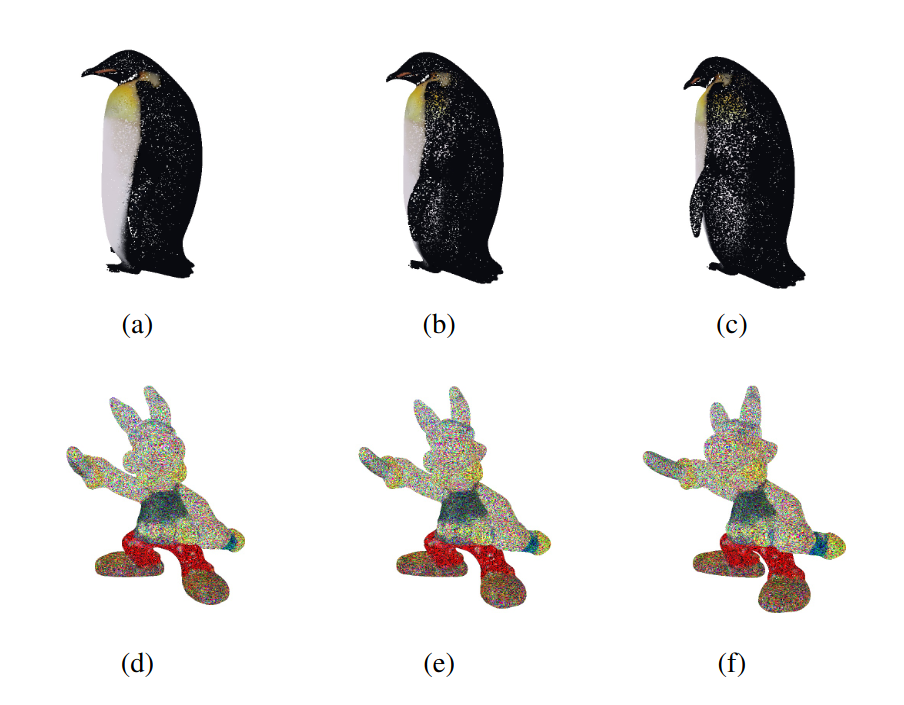
\includegraphics[width=0.75\textwidth]{imagenes/chapter4/ViewPoint}
  \end{center}
  \caption[Ejemplo de distorsiones que se presentan según la perspectiva]{
  Ejemplo de distorsiones que se presentan según la perspectiva.
Vemos que al girar el pingüino se empieza a observar un bajo número de puntos en su 
lateral izquierdo, permitiendo verse a través de él. De forma similar, 
en la imagen de abajo se ve cierta deformación de la cabeza.}
  \label{fig:ViewPoint}
\end{figure}

\begin{figure}
  \begin{center}
    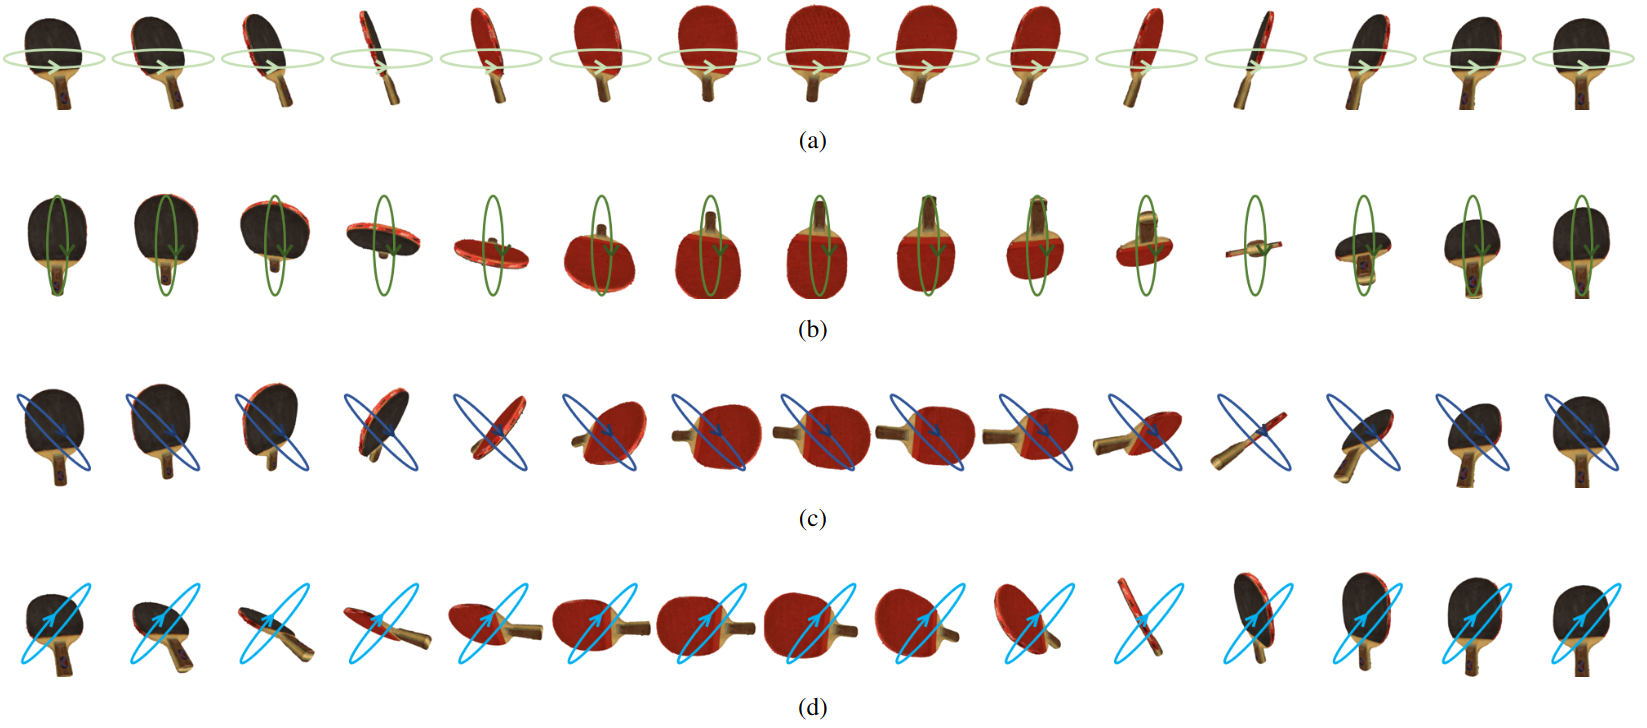
\includegraphics[width=\textwidth]{imagenes/chapter4/VQARotation}
  \end{center}
  \caption[Ejemplo de las rotaciones que utiliza el modelo VQA-PC\cite{VQA-PC}.]
  {Ejemplo de las rotaciones que utiliza el modelo VQA-PC\cite{VQA-PC}.
  Se observa que el final de cualquier eje de rotación es la posición inicial, 
permitiendo así unir suavemente una secuencia de imágenes encadenada de los ejes 
que genere un vídeo de rotación utilizado luego para la estimación.}
  \label{fig:VQARotation}
\end{figure}

Para realizar la secuencia de vídeo, necesitamos realizar correctamente 
el conjunto de rotaciones descritos por las siguientes ecuaciones: 
\begin{equation}
  \theta_A = 
\begin{cases}
\begin{aligned}
   X_\alpha^2 + Y_\alpha^2 & = R^2 \\ 
    Z_\alpha & = 0 
\end{aligned}
\end{cases}
\label{eq:RotationA}
\end{equation}

\begin{equation}
  \theta_B = 
\begin{cases}
\begin{aligned}
   Y_\alpha^2 + Z_\alpha^2 & = R^2 \\ 
    X_\alpha & = 0 
\end{aligned}
\end{cases}
\label{eq:RotationB}
\end{equation}

\begin{equation}
  \theta_C = 
\begin{cases}
\begin{aligned}
   X_\alpha^2 + Y_\alpha^2 + Z_\alpha^2 & = R^2 \\ 
    X_\alpha + Z_\alpha & = 0 
\end{aligned}
\end{cases}
\label{eq:RotationC}
\end{equation}

\begin{equation}
  \theta_D = 
\begin{cases}
\begin{aligned}
   X_\alpha^2 + Y_\alpha^2 + Z_\alpha^2 & = R^2 \\ 
    X_\alpha - Z_\alpha & = 0 
\end{aligned}
\end{cases}
\label{eq:RotationD}
\end{equation}

Y para llevar a cabo la rotación debemos calcular el punto medio de la nube 
de puntos por medio de la siguiente ecuación \eqref{eq:PuntoMedio}:
\begin{equation}
  O_\sigma = \frac{1}{N}\sum_{n=1}^N \sigma_n
  \label{eq:PuntoMedio}
\end{equation}
Donde el $O_\sigma$ representa la coordenada (X,Y,Z) del centro medio de la 
nube de punto, y $\sigma_n$ representa la coordenada del punto $n$-ésimo punto. 
Utilizando ese centro, aplicamos las ecuaciones \eqref{eq:RotationA} a \eqref{eq:RotationD}.

Para extraer las características espaciales empleamos un modelo pre-entrenado, 
en concreto se investigaron variaciones de arquitecturas ResNet\cite{ResNet}. Una 
familia de redes residuales, que en su momento resolvieron el problema 
del estancamiento en el entrenamiento de redes neuronales profundas debido 
a la degradación del gradiente. El único modelo al que optimizaremos sus pesos es 
ResNet, el modelo de extracción temporal solo es un paso previo.

\begin{figure}[htp]
  \begin{center}
    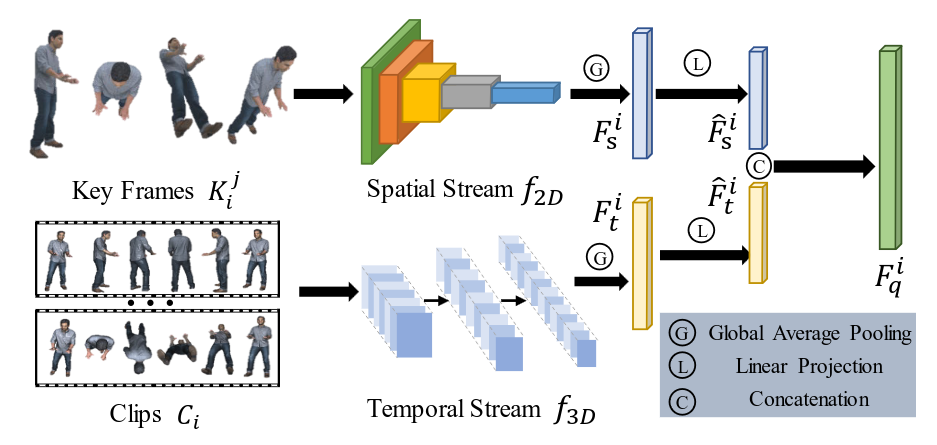
\includegraphics[width=0.65\textwidth]{imagenes/chapter4/PipelineCompleto}
  \end{center}
  \caption{Ejemplo detallado de las etapas del método de VQA-PC}
  \label{fig:VQAPipeline}
\end{figure}

